% !TEX root = USEGUIDE.tex
\pagenumbering{arabic}


\part{Introduction}

    \begin{figure}[H]
    \centering
    \centerline{
\includegraphics[scale=0.2]{LOGO_CLASS.png}}
    \caption{CLASS logo}
    \label{fig:CLASSLogo}
    \end{figure}

    \vspace{2cm}

CLASS stands for \textbf{C}ore \textbf{L}ibrary for \textbf{A}dvanced \textbf{S}cenario \textbf{S}imulation. CLASS is developed from a \textbf{CNRS\footnote{Centre National de la Recherche Scientifique}/IRSN\footnote{Institut de Radioprotection et de S\^{u}ret\'{e} Nucl\'{e}aire}} collaboration started in 2012. It is an \textbf{open source} package of C++ libraries. 
CLASS is a \textbf{dynamical fuel cycle simulation tool}. It allows to \textbf{simulate} the evolution of an entire \textbf{nuclear reactor fleet} and its associated facilities, such as spent fuel pool, fuel fabrication plant, chemical separation plant, disposal and so on. 

Switching from a technology of reactor, or enrichment , or reprocessing,... to an other can strongly impact several quantities such as the resource consumption, waste disposal surface, spent fuel transportation frequency, and so on. The goal of a nuclear fuel cycle code is to calculate nuclei inventories and mass flows evolution in an entire fuel cycle, from the mine to the final disposal in order to \textbf{evaluates the impacts of the changes in a civil nuclear policy of a country}. 

The heart of such codes is located in the treatment of the fuel fabrication and its depletion in reactor. CLASS main asset is its ability to include any kind of reactor, either the system is innovative or standard. Indeed, the opportunity is given to each user to \textbf{build his own reactor model}. CLASS aims to be a useful tool for scenarios studies involving \textbf{Generation IV reactors} transitions as well as innovative fuel cycles, such as the Thorium cycle.



\part{First Steps}
\chapter{Package Content}
The CLASS package contains the followings :
\begin{itemize}
\item   \textbf{data/} : folder containing nuclei properties
\subitem \textbf{FPyield\_Fast\_JEFF3.1.dat }     : file containing fission yield for fast reactors
\subitem \textbf{FPyield\_Thermal\_JEFF3.1.dat}   : file containing fission yield for thermal reactors
\subitem \textbf{Mass.dat }                     : file containing molar masses
\subitem \textbf{SpontaneousFPyield.dat }       : file containing spontaneous fission yields
\subitem \textbf{chart.JEF3T}                   : file containing decay constants and branching ratios

 \item \textbf{DATA\_BASES/}  : this folder contains decay data base and reactor data bases
 \subitem \textbf{DECAY/}     : decay data base
 \subitem \textbf{FBR-Na/}    : Models related to Fast reactor
 \subitem \textbf{PWR/}       : Models related to Pressurised Water Reactor
 
 \item \textbf{documentation/} 
 \subitem \textbf{Manual/}    : folder containing this user guide an its .tex sources
 \subitem \textbf{Doxygen/}   : folder containing the builded doxygen and its generation configuration 

\item \textbf{example/} : folder containing simple examples of CLASS input

\item \textbf{gui/} : folder containing sources of the graphical user interface for CLASS outputs
 \subitem \textbf{bin/}    : folder containing the CLASSGui binary (once comiled)

\item \textbf{lib/} : folder containing the CLASS library (once compiled)
\item \textbf{source/} : folder containing CLASS sources
\subitem \textbf{include/}
\subitem \textbf{Model/} : folder that contain the sources related to the physics models (EquivalenceModel , XSModel and IrradiationModel)
\subitem \textbf{src/}
\item \textbf{Utils/} : folder containing utility software related to reactor data base generation
\subitem \textbf{EQM/} : Example of software to generate equivalence model
\subitem \textbf{MURE2CLASS/} : Software to convert MURE (a fuel depletion code)  output to \hyperref[sec:EvolutionData]{EvolutionData} format
\subitem \textbf{XSM/} : Software to generate cross section predictor
 
 
\end{itemize}

\chapter{Install procedure}

\section{Requirement}
\begin{center}
\begin{minipage}{\textwidth}
\begin{itemize}
\item User skills : Good knowledge of C++. Abilities in using \href{https://root.cern.ch/}{Root}\footnote{https://root.cern.ch/}.
Experience in depletion codes and neutron transport codes.
\item OS : CLASS is known to work under Linux (64  bits) and MacOSX (64 bits). It  has never been tested on any Windows distribution.
\item C++ compiler :  we recommend to use a gnu compiler like gcc4.8 or above.
\item For DARWIN (OSX) users : 
Make sure you have installed XCode and its command line tools (if not dowload and install from AppStore).\\ 
Install \href{http://xquartz.macosforge.org/landing/}{XQuartz}\footnote{http://xquartz.macosforge.org/landing/}.\\
We recommend NOT to use the clang compiler as there is no openmp library in it but the compilation should work with clang anyway\\
TO INSTALL GNU COMPILER : You should install  \href{https://www.macports.org/install.php}{MacPorts}\footnote{https://www.macports.org/install.php} in order to get a gnu compiler.\\
Then types this following command in terminal :\\
\begin{lstlisting}[style=terminal]
sudo port install gcc48
sudo port select --set gcc mp-gcc48
\end{lstlisting}
\item Root (CERN) :  
CLASS uses Root to store output data. 
The graphical user interface CLASSGui is based on Root.
Some algorithms uses the TMVA module of Root. You need to build root from sources with the same C++ compiler as the one you use for CLASS (see first note below). If you prefer use pre-compiled Root libraries, make sure to choose one which is built with the same C++ compiler as the one you will use for compiling CLASS.
For instance if you use a pre-compiled Root libraries compiled with the clang (DARWIN (OSX)) compiler, you have to compile CLASS with clang (and maybe with the same version). 

\end{itemize}
\end{minipage}
\end{center}

\begin{center}
\line(1,0){250}
\end{center}

\begin{large}
\begin{center}
\textbf{IMPORTANT NOTES : } \\
\vspace{0.5cm}
\textbf{about building Root from sources} \\
\end{center}
\end{large} 
\underline{For OSX users (tested with OSX Yosemite \& gcc5 from macport) :}\\
With terminal, go to the unziped ROOT directory then :
\begin{lstlisting}[style=terminal]
./configure --with-cxx=/opt/local/bin/g++ --with-cc=/opt/local/bin/gcc --with-f77=/opt/local/bin/gfortran --with-ld=/opt/local/bin/g++ --enable-builtin-freetype --disable-cocoa --enable-minuit2 --disable-bonjour
\end{lstlisting}
If configuration succeed :
\begin{lstlisting}[style=terminal]
make -j
\end{lstlisting}
\vspace{0.5cm}
\underline{For Linux users :}\\
\begin{lstlisting}[style=terminal]
./configure 
make -j
\end{lstlisting}
seems to work easily
\vspace{1cm}

\begin{large}
\begin{center}
\textbf{about the Root version to use} \\
\end{center}
\end{large} 

The version 6.00 and above doesn't use the CINT environment annymore. As a consequence, CLASS is not able to use these new Root versions. You have to use an older one.
Root package of version 5.34/26 and older have a memory leak issue when using TMVA leading to a \textbf{freeze of your computer.}
Compatible versions of Root are : 
\begin{equation}
\text{Root v5.34/30} \leq \text{Working Root version} \leq \text{Root v5.99/06}
\end{equation}

You can use an older Root version as v5.34/30 but you have to make this modification in the sources :
Open with your favourite text editor the file  \$ROOTSYS/tmva/src/Reader.cxx (\$ROOTSYS is the path to your ROOT installation folder) and replace the following :\\

\begin{center}
\begin{minipage}{\textwidth}
\begin{lstlisting}[style=customc]
TMVA::Reader::~Reader( void )
{
   // destructor

   delete fDataSetManager; // DSMTEST

   delete fLogger;
}
\end{lstlisting}
\end{minipage}
\end{center}

by :\\
\begin{center}
\begin{minipage}{\textwidth}
\begin{lstlisting}[style=customc]
TMVA::Reader::~Reader( void )
{
   // destructor
   std::map<TString, IMethod* >::iterator itr;
   for( itr = fMethodMap.begin(); itr != fMethodMap.end(); itr++) {
      delete itr->second;
   }
   fMethodMap.clear();

   delete fDataSetManager; // DSMTEST

   delete fLogger;
}
\end{lstlisting}
\end{minipage}
\end{center}

then type in your terminal : 

\begin{center}
\begin{minipage}{\textwidth}
\begin{lstlisting}[style=terminal]
cd $ROOTSYS
sudo make -j
\end{lstlisting}
\end{minipage}
\end{center}

\begin{center}
\line(1,0){250}
\end{center}


\section{Installation}
Decompress the CLASS.tar.gz in your wanted location. 

 Then type in terminal:
\begin{center}
\begin{minipage}{\textwidth}
\begin{lstlisting}[style=terminal]
cd < CLASS root folder >
./install.sh --help
\end{lstlisting}
\end{minipage}
\end{center}

You should have in terminal the help of CLASS install script :
\begin{center}
\begin{minipage}{\textwidth}
\begin{lstlisting}[style=terminal]
###############################################################
############## configures and compiles CLASS V4.1 #############
###############################################################

Usage: install.sh [VAR=VALUE] [OPTION]
Defaults for the options are specified in brackets.

Configuration:
  -h, --help         display this help and exit
Optional Features:
  --disable-OMP      do not compile with OpenMP support for evolution 
                     [default: enable for gcc version >= 4.1]
  --InstallLib-path=path     Location of made CLASS's libraries [default= $PWD/lib]

Some influential environment variables:
  CXX         C++ compiler command [default=g++]
  CXXFLAGS    C++ compiler flags, e.g. -I<include dir> if
              you have headers in a nonstandard directory <include dir>
  CPPFLAGS    C++ preprocessor flags, e.g. -D<special flag>

Report bugs to <leniau@subatech.in2p3.fr>.
(special thanks to PTO)
\end{lstlisting}
\end{minipage}
\end{center}
We suggest to use the default install by typing :
\begin{center}
\begin{minipage}{\textwidth}
\begin{lstlisting}[style=terminal]
./install.sh
\end{lstlisting}
\end{minipage}
\end{center}
This script (used without argument) will compile and install CLASS libraries in < CLASS root folder >/lib.
It will build CLASSGui binary in < CLASS root folder >/gui/bin/.It will set the correct pathway for the decay data base and add the CLASS environment variables in your \$HOME/.(shell)rc. With (shell) is your default shell. If everything goes well, you should see in terminal something like (see next page) and be able to compile your first CLASS input:
\begin{center}
\begin{minipage}{\textwidth}
\begin{lstlisting}[style=terminal]
Checking for ROOT cern lib... yes
Checking for omp.h... yes
   You can disable the use of this library with "--disable-OMP" option
Building Librairies Folder @ /scratch/leniau/App/local/CLASS_Support/lib
####################################################
######### Compilation of CLASS libraries ###########
####################################################
[...]
libCLASSpkg.so done
[...]
libCLASSpkg_root.so done
####################################################
########## Compilation Done  #######################
####################################################
MURE libraries installed in
----> /scratch/leniau/App/local/CLASS_Support/lib
####################################################
######### Compilation of CLASSGUI binary ###########
####################################################
[...]
CLASSGui is now available in /scratch/leniau/App/local/CLASS_Support/gui/bin 
####################################################
########## Compilation Done  #######################
####################################################
####################################################
########## SET DECAY DATA BASES PATHES #############
####################################################
-> Done
/scratch/leniau/App/local/CLASS_Support
####################################################
########## ENVIRONEMENT VARIABLES ##################
####################################################
-> Your default shell is : /bin/tcsh
-> Your .tcshrc will be edited if CLASS_PATH CLASS_include
   and CLASS_lib aren't defined yet 

CHECKING LOADED ENVIRONEMENT VARIABLES ............
Not found in your loaded .tcshrc. 
Setting variables ...

PRESS ENTER IF DEFAULT IS CORRECT
====>ENTER THE PATH TO THE CLASS root folder (defalut /scratch/leniau/App/local/CLASS_Support) 
Path of the CLASS include folder is /scratch/leniau/App/local/CLASS_Support

====>ENTER THE PATH TO THE CLASS INCLUDE (default: /scratch/leniau/App/local/CLASS_Support/source/include/): 
Path of the CLASS include folder is /scratch/leniau/App/local/CLASS_Support/source/include/

====>ENTER THE PATH WHERE CLASS LIB ARE INSTALLED (default: /scratch/leniau/App/local/CLASS_Support/lib): 
Path of the CLASS lib folder is /scratch/leniau/App/local/CLASS_Support/lib

Environnment variables added in /Users/leniau/.tcshrc
LOADING /Users/leniau/.tcshrc ... done

!!!!!!!!!!!!!!!!!!!!!!!!!!!!!!!!!!!!!!!!!!!!!!!!!!!!!!!!!!!!
 Congratulations you are now able to compile your first     
               CLASS .cxx input.                            
 Please read /scratch/leniau/App/local/CLASS_Support/documentation/Manual/USEGUIDE.pdf
 !!!!!!!!!!!!!!!!!!!!!!!!!!!!!!!!!!!!!!!!!!!!!!!!!!!!!!!!!!!!
\end{lstlisting}
\end{minipage}
\end{center}

Please report installation issue to the \href{https://forge.in2p3.fr/projects/classforge/issues/new}{forge}\footnote{https://forge.in2p3.fr/projects/classforge/issues/new}.

\chapter{CLASS Execution}
CLASS is a set of C++ libraries, there is no CLASS binary file. A CLASS executable has to be build by user using objects and methods defined in the CLASS package. \\
The compilation line for generating your executable from a .cxx file is the following :
(You can find CLASS input examples in \$CLASS\_PATH/example/)

\begin{center}
\begin{minipage}{\textwidth}
\begin{lstlisting}[style=terminal]
g++ -o CLASS_exec YourScenario.cxx -I $CLASS_include -L $CLASS_lib -lCLASSpkg `root-config --cflags` `root-config --libs` -fopenmp -lgomp -Wunused-result -lTMVA
\end{lstlisting}
\end{minipage}
\end{center}
Then type 
\begin{center}
\begin{minipage}{\textwidth}
\begin{lstlisting}[style=terminal]
./CLASS_exec
\end{lstlisting}
\end{minipage}
\end{center}

The following should show in your terminal :

    \begin{figure}[H]
    \centering
    \centerline{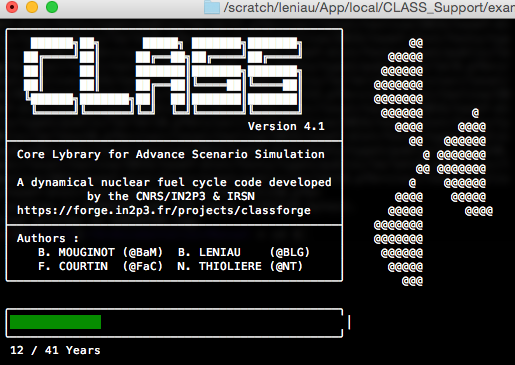
\includegraphics[scale=0.9]{CLASS_Run.png}}
    \caption{CLASS logo}
    \label{fig:CLASSLogo}
    \end{figure}




\chapter{News, forum, troubleshooting, doxygen ...}
CLASS has a \href{https://forge.in2p3.fr/projects/classforge}{forge}\footnote{https://forge.in2p3.fr/projects/classforge} hosted by the IN2P3  where you can find :

\begin{itemize}
\item \href{https://forge.in2p3.fr/projects/classforge/boards}{A forum}\footnote{https://forge.in2p3.fr/projects/classforge/boards} where you are invited to post your trouble about CLASS installation and usage. You may find the answer to your trouble on a already posted thread.
\item \href{https://forge.in2p3.fr/projects/classforge/embedded/doxygen/inherits.html}{A doxygen}\footnote{https://forge.in2p3.fr/projects/classforge/embedded/doxygen/inherits.html} where all the CLASS objects and methods are defined and explained. Note that the doxygen is also contained in \$CLASS\_PATH/documentation/doxygen/CLASSDoxygen.html
\item \href{https://forge.in2p3.fr/projects/classforge/news}{News}\footnote{https://forge.in2p3.fr/projects/classforge/news} : All the news related to CLASS
\end{itemize}
A \href{classuser-l@ccpntc02.in2p3.fr}{Mailing List}\footnote{classuser-l@ccpntc02.in2p3.fr} also exist in order to be warned of all the change inside CLASS and to allow user to exchange directly on the code. One can join the mailing list through the following  \href{http://listserv.in2p3.fr/cgi-bin/wa?SUBED1=classuser-l&A=1}{link}\footnote{http://listserv.in2p3.fr/cgi-bin/wa?SUBED1=classuser-l\&A=1}.



